\documentclass{wssci}
\usepackage{amssymb}
\usepackage{amsmath}
\usepackage{subfigure}
\usepackage{fancyhdr}
\usepackage{color}
\usepackage{xcolor}
\usepackage{graphicx}
\usepackage{bm}
\usepackage{yhmath}
\usepackage{multirow}
\usepackage{cleveref}
\pagestyle{fancyplain}
\usepackage{epstopdf}
\lhead{ \fancyplain{}{Sub Topic: Laminar Flames} }
\rhead{ \fancyplain{}{} }
\begin{document}

\title{Stabilization of laminar nonpremixed DME/air coflow flames at elevated temperature and pressure}

\author{
%
% Insert the author names below
Sili Deng, Peng Zhao, Michael E. Mueller*, Chung K. Law 
%
}
\date{
% This is actually the contacts.
Department of Mechanical and Aerospace Engineering\\
Princeton University, Princeton, NJ 08544, USA\\
*Corresponding Author Email: muellerm@princeton.edu
%
}

\maketitle
\thispagestyle{fancyplain}
%====================================================================

\begin{abstract}
\textbf{Abstract:} The structure and stabilization mechanism of laminar nonpremixed autoignitive DME/air coflow flames were investigated at elevated temperature and pressure. Computations with detailed chemistry were performed for DME and heated coflow air at $30$ atm, with uniform inlet velocities ($2.4$, $3.2$, and $8.0$ m/s) imposed for both streams.  The heat release rate profiles were first examined for each case to demonstrate the multibrachial thermal structure.  Species concentrations and temperature were sampled along mixture fraction iso-contours, and Chemical Explosive Mode Analysis (CEMA) was performed to identify the controlling chemistry at representative points.  One-dimensional Lagrangian Flamelet Analysis (LFA) was also performed and compared with the two-dimensional computations to elucidate the relative importance of diffusion processes parallel and perpendicular to the mixture fraction gradient.  Various coflow temperatures with different inlet velocities were examined to elucidate their influences on the multibrachial structure, as well as the stabilization mechanism.  It is found that at high coflow boundary temperature or low inlet velocity, the classical tribrachial flame structure was first achieved, and autoignition contributed less to the stabilization due to reduced lift-off height and therefore limited residence time.  The kinematic balance between the flow speed and flame propagation speed is the dominant stabilization mechanism.  On the contrary, kinetic stabilization was achieved at lower coflow temperature or higher inlet velocity, as inhomogeneous autoignition became dominant.  The transition of different stabilization mechanisms can be made by changing either the chemical time or residence time of the system.  Based on these results, a regime diagram is constructed that identifies the possible stabilization regimes: blow-off, kinetically stabilized, autoignition-propagation-coupled stabilized, kinematically stabilized, and burner stabilized regimes.\\
\textbf{\textit{Keyword: Stabilization, Nonpremixed coflow flame, Autoignition, Dimethyl ether (DME)}}
\end{abstract}

%====================================================================

\section{Introduction}

Nonpremixed laminar lifted flames have been extensively investigated~\cite{chung07}.  A two-dimensional tribrachial structure (also known as triple flame)~\cite{buckmaster02} is observed, due to the partially premixing of the fuel and oxidizer.  Specifically, a lean, a rich premixed flame wing, and a trailing diffusion flame tail intersect at the triple point, which is generally considered as the stabilization point.  Under nonautoignitive conditions, the local flame propagation speed balances the incoming flow speed, and this dynamic balance is characterized as the stabilization mechanism.  As reviewed by Chung~\cite{chung07}, burned gas expansion~\cite{ruetsch95,lee97,plessing98,kioni99}, concentration gradient~\cite{dold89,hartley91,ghosal00}, and velocity gradient~\cite{kim07} influence the local flame speed as well as flow field and therefore affect the stabilization, propagation, and instability of tribrachial flames.

However, practical diesel engines and gas turbines are operated at elevated pressures and temperatures to improve efficiency.  As a consequence, autoignition is activated, and the thermal and chemical structure of the tribrachial flame, as well as the stabilization mechanism could be affected by the autoignition process.  Furthermore, the autoignition process for most large hydrocarbons used in practical engines consists of two stages.  Low temperature chemistry is dominant in the first stage ignition, and high temperature chemistry is responsible for the second ignition stage.  The transition of the ignition chemistry in the intermediate temperature regime results in the negative temperature coefficient (NTC) phenomenon, as the overall ignition delay time increases as the initial temperature increases.  The NTC phenomenon is responsible for engine knock and has been extensively studied in homogeneous systems~\cite{zador11}.  As Law and co-workers~\cite{law12,zhao13,deng14} recently demonstrated, nonpremixed flame ignition characteristics can also be affected by NTC effects, especially at elevated pressures.  These computational and experimental studies were conducted in the nonpremixed counterflow system, where the transport time scale is well characterized.  When the transport and NTC chemistry time scales are comparable, the two processes are strongly coupled, and the inhomogeneous autoignition process is modified by NTC chemistry.

To study the autoignition with NTC chemistry effects on nonpremixed lifted flame stabilization, Krisman~\emph{et al.}~\cite{krisman14} recently conducted a numerical study of dimethyl ether (DME)/air at $40$ atmospheres and elevated air coflow temperatures ($700-1500$ K) and observed multibrachial thermal structures.  The autoignition response in the two-dimensional computation was compared with the homogeneous autoignition under the same initial conditions.  A transported budget analysis of methoxymethylperoxy (CH$_3$OCH$_2$O$_2$) and hydroxyl (OH) radical, which represent the low and high temperature chemistry, respectively, was performed to differentiate deflagration from autoignition.  

To further elucidate the chemical structure of the multibrachial structure and the roles of autoignition and flame chemistry in the stabilization mechanism, a recent numerical study by the authors~\cite{deng15} was performed in a nonpremixed DME/air coflow configuration at elevated temperature and pressure.  Chemical Explosive Mode Analysis (CEMA) was adopted to identify locally dominant reactions and demonstrate the dominant combustion mode.  In addition, Lagrangian Flamelet Analysis (LFA) was adopted to differentiate the transport parallel and perpendicular to mixture fraction gradient and elucidate the dominant stabilization mechanism.  The transitions of the stabilization mechanism were demonstrated, as the coflow boundary temperature increases, while the uniform inlet velocities kept constant.

In the present study, nonpremixed DME/air coflow flames were further studied at elevated temperature and pressure.  Residence time effects on the stabilization regimes were examined by varying the uniform inlet velocities, while the coflow temperature kept constant.  Moreover, the coupling between autoignition and flame chemistry was examined with CEMA and LFA to demonstrate the transition between different stabilization regimes.                         
%====================================================================

\section{Computational Details}

The axisymmetric DME stream at $300$ K was surrounded by heated coflow air at $30$ atmospheres.  The fuel nozzle diameter $D$ is $0.8$ mm, and the fuel and air are initially separated with a wall with thickness $D/20$.  The diameter of the coflow is $3.9$ mm with slip wall boundary condition.  This diameter was made wide enough that further increase did not influence the computation results.  Uniform inlet velocities for both streams were specified, outflow boundary condition was specified for the exit.  

The governing equations, transport, and chemical models were adopted the same as in Deng~\emph{et al.}~\cite{deng15}.  In brief, the Navier-Stokes equation with buoyancy in the streamwise direction and the conservation equations of mass, species, and energy were solved.  The species diffusivities are determined from a constant, nonunity Lewis number.  The conserved scalar mixture fraction $Z$ is specified as unity and zero for the fuel stream and coflow at the inlet, respectively, and computed by solving its transport equation with unity Lewis number~\cite{pitsch98b}.  A DME skeletal mechanism of $39$ species~\cite{bhagatwala15}, which was reduced from the well validated detailed mechanism of Zhao \emph{et al.}~\cite{zhao08}, was adopted as the chemical model.

The governing equations with low-Mach number formulation is solved using NGA, based on the numerical methods of Desjardins \emph{et al.}~\cite{desjardins08}.  The momentum and scalar equations are discretized with a second-order centered scheme and a third-order WENO scheme~\cite{liu94}, respectively, on a staggered mesh.  The iterative second-order semi-implicit Crank-Nicolson scheme of Pierce and Moin~\cite{pierce01} is adopted for temporal integration.  The chemical source terms for species and energy equations are evaluated independently from the transport terms using the CVODE package~\cite{cohen96}.

According to the previous grid convergence study~\cite{deng15}, uniform grid spacing in the axial direction was set as $\Delta x = 2.2-4.8$ $\mu$m.  Nonuniform grid spacing in the radial direction was set as $\Delta r = 2.5$ $\mu$m for the minima, and the grid stretch rate was less than $3$\%.    
%====================================================================
\section{Residence Time Effects}

The residence time effects on the nonpremixed coflow flame stabilization were demonstrated by fixing the coflow temperature at $900$ K, while varying the uniform inlet velocities as $2.4$, $3.2$, and $8.0$ m/s.  The $3.2$ m/s case was reproduced as in the previous work~\cite{deng15}.  Details about the numerical discretization are summarized in Table.~\ref{table:domain_V}.

\begin{table*}
  \caption{Computational domain and number of grid points.}
  \label{table:domain_V}
  \centering
  \normalsize
  \resizebox{0.4\textwidth}{!}{
  \begin{tabular}{lc*{2}{c}}
    \hline
    Inlet Velocity [m/s]& $2.4$  & $3.2$  & $8.0$   \\
    \hline
    Length [mm]& $3.5$ & $3.5$ & $15$\\
    %Coflow O.D. [mm]& $3.9$ & $3.9$ & $3.9$\\
    $N_x$ & $1536$ & $1536$  & $3072$\\
    $N_r$ & $176$ & $176$ & $176$\\
    \hline
   \end{tabular}
}
\end{table*}

\subsection{Thermal and Chemical Structure}  
The heat release rate profiles for the three cases are shown in Fig.~\ref{fig:HRR_V}.  A qualitative determination of the stabilization point is the most upstream point on the largest heat release contour (the leading point), colored by red.  The mixture fraction iso-contours of $Z_{\rm st} = 0.1005$, $Z = 0.2$, and $Z = 0.3$ are delineated in solid black lines, from right to left.

When the inlet velocity is the lowest, $2.4$ m/s, a tribrachial thermal structure is observed, very similar to the classical triple flame.  The triple point, where the three large heat release branches intersect, is also the stabilization point.  Some heat release can be found upstream of the tribrachial thermal structure, due to the partially reacting mixture at elevated temperature, but is much less than the heat release from the flame structure. 

As the inlet velocity increases to $3.2$ m/s, another branch with large heat release is found attached to the tribrachial structure, around $Z = 0.2$.  The stabilization point is again the same as the triple point.  This structure has been analyzed in the previous work by the authors~\cite{deng15}.

As the inlet velocity further increases to $8.0$ m/s, the stabilization point does not locate on the tribrachial structure any more.  Instead, it locates near $Z = 0.25$ and is the intersection point of two trailing heat release branches.  Attached to the leaner branch, there is a tribrachial structure, similar to the triple flame structure.  This multibrachial structure looks the same as the $800$ K case with lower inlet velocity in the authors' previous work~\cite{deng15}.

\begin{figure}
  \centering
  \scriptsize
  \vspace{-0.1in}
  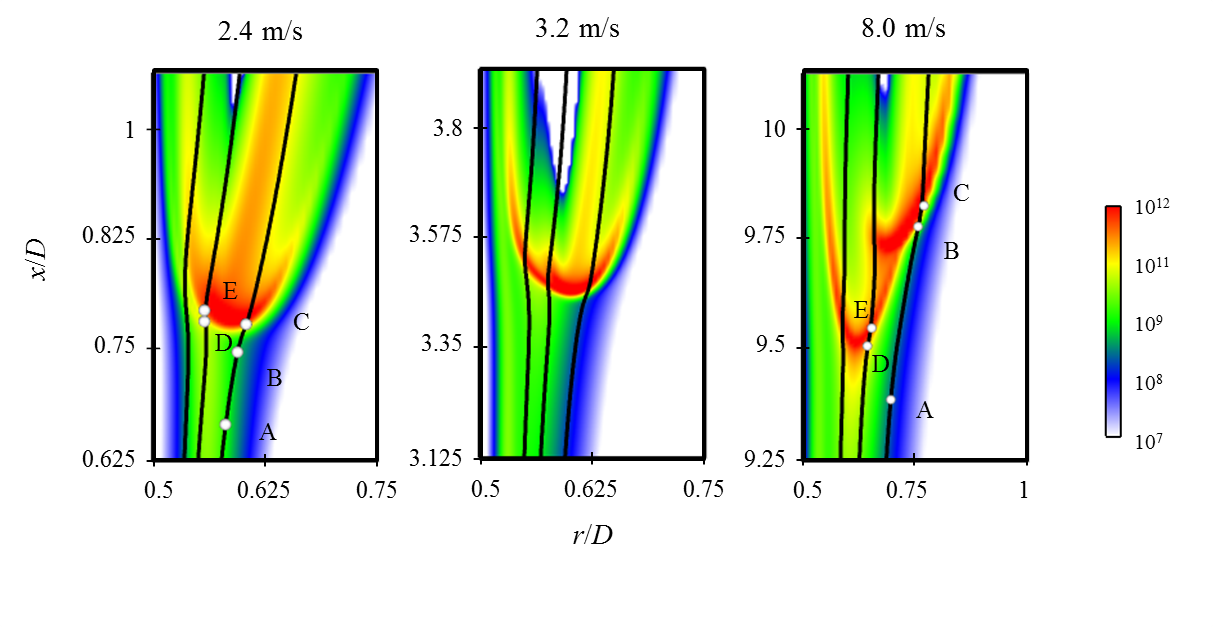
\includegraphics[width=0.7\textwidth]{HRR_V.png}
  \normalsize
  \vspace{-0.4in}
  \caption{Heat release rate [J/m$^3$-s] profiles.  The iso-contours of $Z_{\rm st}$, $Z = 0.2$, and $Z = 0.3$ are outlined from right to left in solid lines, respectively.  The CEMA sampling points for $2.4$ and $8.0$ m/s cases are marked along the iso-contours.}
  \label{fig:HRR_V}
\end{figure}

The controlling chemistry of the three cases were studied with Chemical Explosive Mode Analysis (CEMA)~\cite{lu10,shan12}.   Briefly, local species concentrations and temperature are sampled from the two-dimensional computation and feed into CEMA to evaluate the eigenvalues of the Jacobian matrix of the chemical source terms.  The largest positive eigenvalue, which is defined as the chemical explosive mode, describes the rate of system runaway.  The projection of a reaction on the explosive mode is defined as the explosion participation index to account for its contribution to the explosive mode.

In the present study, such samplings were conducted along $Z_{\rm st}$, $Z = 0.2$, and $Z = 0.3$ iso-contours, as shown in Fig.~\ref{fig:HRR_V}.  Based on the explosive mode and participation index, the evolution of the dominant reactions are shown in Fig.~\ref{fig:CEMA_V}.

\begin{figure}
  \centering
  \scriptsize
  \resizebox{0.8\textwidth}{!}{% GNUPLOT: LaTeX picture with Postscript
\begingroup
  \makeatletter
  \providecommand\color[2][]{%
    \GenericError{(gnuplot) \space\space\space\@spaces}{%
      Package color not loaded in conjunction with
      terminal option `colourtext'%
    }{See the gnuplot documentation for explanation.%
    }{Either use 'blacktext' in gnuplot or load the package
      color.sty in LaTeX.}%
    \renewcommand\color[2][]{}%
  }%
  \providecommand\includegraphics[2][]{%
    \GenericError{(gnuplot) \space\space\space\@spaces}{%
      Package graphicx or graphics not loaded%
    }{See the gnuplot documentation for explanation.%
    }{The gnuplot epslatex terminal needs graphicx.sty or graphics.sty.}%
    \renewcommand\includegraphics[2][]{}%
  }%
  \providecommand\rotatebox[2]{#2}%
  \@ifundefined{ifGPcolor}{%
    \newif\ifGPcolor
    \GPcolortrue
  }{}%
  \@ifundefined{ifGPblacktext}{%
    \newif\ifGPblacktext
    \GPblacktexttrue
  }{}%
  % define a \g@addto@macro without @ in the name:
  \let\gplgaddtomacro\g@addto@macro
  % define empty templates for all commands taking text:
  \gdef\gplbacktext{}%
  \gdef\gplfronttext{}%
  \makeatother
  \ifGPblacktext
    % no textcolor at all
    \def\colorrgb#1{}%
    \def\colorgray#1{}%
  \else
    % gray or color?
    \ifGPcolor
      \def\colorrgb#1{\color[rgb]{#1}}%
      \def\colorgray#1{\color[gray]{#1}}%
      \expandafter\def\csname LTw\endcsname{\color{white}}%
      \expandafter\def\csname LTb\endcsname{\color{black}}%
      \expandafter\def\csname LTa\endcsname{\color{black}}%
      \expandafter\def\csname LT0\endcsname{\color[rgb]{1,0,0}}%
      \expandafter\def\csname LT1\endcsname{\color[rgb]{0,1,0}}%
      \expandafter\def\csname LT2\endcsname{\color[rgb]{0,0,1}}%
      \expandafter\def\csname LT3\endcsname{\color[rgb]{1,0,1}}%
      \expandafter\def\csname LT4\endcsname{\color[rgb]{0,1,1}}%
      \expandafter\def\csname LT5\endcsname{\color[rgb]{1,1,0}}%
      \expandafter\def\csname LT6\endcsname{\color[rgb]{0,0,0}}%
      \expandafter\def\csname LT7\endcsname{\color[rgb]{1,0.3,0}}%
      \expandafter\def\csname LT8\endcsname{\color[rgb]{0.5,0.5,0.5}}%
    \else
      % gray
      \def\colorrgb#1{\color{black}}%
      \def\colorgray#1{\color[gray]{#1}}%
      \expandafter\def\csname LTw\endcsname{\color{white}}%
      \expandafter\def\csname LTb\endcsname{\color{black}}%
      \expandafter\def\csname LTa\endcsname{\color{black}}%
      \expandafter\def\csname LT0\endcsname{\color{black}}%
      \expandafter\def\csname LT1\endcsname{\color{black}}%
      \expandafter\def\csname LT2\endcsname{\color{black}}%
      \expandafter\def\csname LT3\endcsname{\color{black}}%
      \expandafter\def\csname LT4\endcsname{\color{black}}%
      \expandafter\def\csname LT5\endcsname{\color{black}}%
      \expandafter\def\csname LT6\endcsname{\color{black}}%
      \expandafter\def\csname LT7\endcsname{\color{black}}%
      \expandafter\def\csname LT8\endcsname{\color{black}}%
    \fi
  \fi
  \setlength{\unitlength}{0.0500bp}%
  \begin{picture}(7200.00,5040.00)%
    \gplgaddtomacro\gplbacktext{%
      \csname LTb\endcsname%
      \put(2748,1043){\makebox(0,0)[r]{\strut{}CH$_3$OCH$_2$+O$_2$$\Longleftrightarrow$CH$_3$OCH$_2$O$_2$}}%
      \put(2748,1383){\makebox(0,0)[r]{\strut{}CH$_2$OCH$_2$O$_2$H$\Longleftrightarrow$OH+CH$_2$O+CH$_2$O}}%
      \put(2748,1722){\makebox(0,0)[r]{\strut{}CH$_3$OCH$_3$+OH$\Longleftrightarrow$CH$_3$OCH$_2$+H$_2$O}}%
      \put(2748,2061){\makebox(0,0)[r]{\strut{}H+O$_2$+M$\Longleftrightarrow$HO$_2$+M}}%
      \put(2748,2400){\makebox(0,0)[r]{\strut{}HCO+O$_2$$\Longleftrightarrow$CO+HO$_2$}}%
      \put(2748,2740){\makebox(0,0)[r]{\strut{}CH$_3$OCH$_2$O$_2$$\Longleftrightarrow$CH$_2$OCH$_2$O$_2$H}}%
      \put(2748,3079){\makebox(0,0)[r]{\strut{}CH$_2$O+OH$\Longleftrightarrow$HCO+H$_2$O}}%
      \put(2748,3418){\makebox(0,0)[r]{\strut{}HO$_2$CH$_2$OCHO$\Longleftrightarrow$OCH$_2$OCHO+OH}}%
      \put(2748,3757){\makebox(0,0)[r]{\strut{}CH$_2$O+H$\Longleftrightarrow$HCO+H$_2$}}%
      \put(2748,4097){\makebox(0,0)[r]{\strut{}CH$_3$OCH$_3$+H$\Longleftrightarrow$CH$_3$OCH$_2$+H$_2$}}%
      \put(2748,4436){\makebox(0,0)[r]{\strut{}H+O$_2$$\Longleftrightarrow$O+OH}}%
      \put(2880,484){\makebox(0,0){\strut{}-1}}%
      \put(3861,484){\makebox(0,0){\strut{}-0.5}}%
      \put(4842,484){\makebox(0,0){\strut{} 0}}%
      \put(5822,484){\makebox(0,0){\strut{} 0.5}}%
      \put(6803,484){\makebox(0,0){\strut{} 1}}%
      \csname LTb\endcsname%
      \put(4841,154){\makebox(0,0){\strut{}Normalized Participation Index}}%
      \put(5234,1332){\makebox(0,0)[l]{\strut{}Point A}}%
      \put(5234,1501){\makebox(0,0)[l]{\strut{}Point B}}%
      \put(5234,1688){\makebox(0,0)[l]{\strut{}Point C}}%
      \put(5234,1857){\makebox(0,0)[l]{\strut{}Point D}}%
      \put(5234,2027){\makebox(0,0)[l]{\strut{}Point E}}%
      \put(5234,2231){\makebox(0,0)[l]{\strut{}$2.4$ m/s}}%
    }%
    \gplgaddtomacro\gplfronttext{%
      \csname LTb\endcsname%
      \put(5690,1337){\makebox(0,0)[r]{\strut{} }}%
      \csname LTb\endcsname%
      \put(5690,1513){\makebox(0,0)[r]{\strut{} }}%
      \csname LTb\endcsname%
      \put(5690,1689){\makebox(0,0)[r]{\strut{} }}%
      \csname LTb\endcsname%
      \put(5690,1865){\makebox(0,0)[r]{\strut{} }}%
      \csname LTb\endcsname%
      \put(5690,2041){\makebox(0,0)[r]{\strut{} }}%
    }%
    \gplbacktext
    \put(0,0){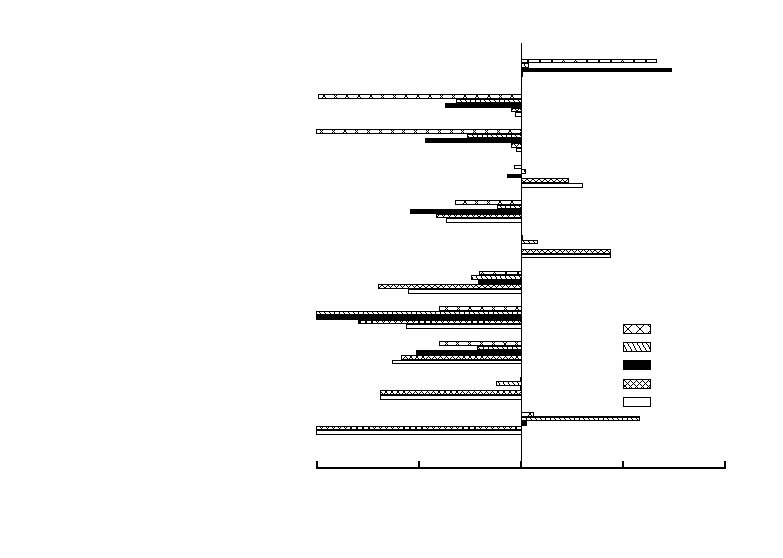
\includegraphics{ch-dynamics/CEMA_24}}%
    \gplfronttext
  \end{picture}%
\endgroup
}
  \resizebox{0.8\textwidth}{!}{% GNUPLOT: LaTeX picture with Postscript
\begingroup
  \makeatletter
  \providecommand\color[2][]{%
    \GenericError{(gnuplot) \space\space\space\@spaces}{%
      Package color not loaded in conjunction with
      terminal option `colourtext'%
    }{See the gnuplot documentation for explanation.%
    }{Either use 'blacktext' in gnuplot or load the package
      color.sty in LaTeX.}%
    \renewcommand\color[2][]{}%
  }%
  \providecommand\includegraphics[2][]{%
    \GenericError{(gnuplot) \space\space\space\@spaces}{%
      Package graphicx or graphics not loaded%
    }{See the gnuplot documentation for explanation.%
    }{The gnuplot epslatex terminal needs graphicx.sty or graphics.sty.}%
    \renewcommand\includegraphics[2][]{}%
  }%
  \providecommand\rotatebox[2]{#2}%
  \@ifundefined{ifGPcolor}{%
    \newif\ifGPcolor
    \GPcolortrue
  }{}%
  \@ifundefined{ifGPblacktext}{%
    \newif\ifGPblacktext
    \GPblacktexttrue
  }{}%
  % define a \g@addto@macro without @ in the name:
  \let\gplgaddtomacro\g@addto@macro
  % define empty templates for all commands taking text:
  \gdef\gplbacktext{}%
  \gdef\gplfronttext{}%
  \makeatother
  \ifGPblacktext
    % no textcolor at all
    \def\colorrgb#1{}%
    \def\colorgray#1{}%
  \else
    % gray or color?
    \ifGPcolor
      \def\colorrgb#1{\color[rgb]{#1}}%
      \def\colorgray#1{\color[gray]{#1}}%
      \expandafter\def\csname LTw\endcsname{\color{white}}%
      \expandafter\def\csname LTb\endcsname{\color{black}}%
      \expandafter\def\csname LTa\endcsname{\color{black}}%
      \expandafter\def\csname LT0\endcsname{\color[rgb]{1,0,0}}%
      \expandafter\def\csname LT1\endcsname{\color[rgb]{0,1,0}}%
      \expandafter\def\csname LT2\endcsname{\color[rgb]{0,0,1}}%
      \expandafter\def\csname LT3\endcsname{\color[rgb]{1,0,1}}%
      \expandafter\def\csname LT4\endcsname{\color[rgb]{0,1,1}}%
      \expandafter\def\csname LT5\endcsname{\color[rgb]{1,1,0}}%
      \expandafter\def\csname LT6\endcsname{\color[rgb]{0,0,0}}%
      \expandafter\def\csname LT7\endcsname{\color[rgb]{1,0.3,0}}%
      \expandafter\def\csname LT8\endcsname{\color[rgb]{0.5,0.5,0.5}}%
    \else
      % gray
      \def\colorrgb#1{\color{black}}%
      \def\colorgray#1{\color[gray]{#1}}%
      \expandafter\def\csname LTw\endcsname{\color{white}}%
      \expandafter\def\csname LTb\endcsname{\color{black}}%
      \expandafter\def\csname LTa\endcsname{\color{black}}%
      \expandafter\def\csname LT0\endcsname{\color{black}}%
      \expandafter\def\csname LT1\endcsname{\color{black}}%
      \expandafter\def\csname LT2\endcsname{\color{black}}%
      \expandafter\def\csname LT3\endcsname{\color{black}}%
      \expandafter\def\csname LT4\endcsname{\color{black}}%
      \expandafter\def\csname LT5\endcsname{\color{black}}%
      \expandafter\def\csname LT6\endcsname{\color{black}}%
      \expandafter\def\csname LT7\endcsname{\color{black}}%
      \expandafter\def\csname LT8\endcsname{\color{black}}%
    \fi
  \fi
  \setlength{\unitlength}{0.0500bp}%
  \begin{picture}(7200.00,5040.00)%
    \gplgaddtomacro\gplbacktext{%
      \csname LTb\endcsname%
      \put(2748,1043){\makebox(0,0)[r]{\strut{}H$_2$O$_2$+M$\Longleftrightarrow$OH+OH+M}}%
      \put(2748,1383){\makebox(0,0)[r]{\strut{}HCO+O$_2$$\Longleftrightarrow$CO+HO$_2$}}%
      \put(2748,1722){\makebox(0,0)[r]{\strut{}CH$_2$O+OH$\Longleftrightarrow$HCO+H$_2$O}}%
      \put(2748,2061){\makebox(0,0)[r]{\strut{}HO$_2$+HO$_2$$\Longleftrightarrow$H$_2$O$_2$+O$_2$}}%
      \put(2748,2400){\makebox(0,0)[r]{\strut{}CH$_3$OCH$_3$+HO$_2$$\Longleftrightarrow$CH$_3$OCH$_2$+H$_2$O$_2$}}%
      \put(2748,2740){\makebox(0,0)[r]{\strut{}CH$_3$OCH$_2$O$_2$$\Longleftrightarrow$CH$_2$OCH$_2$O$_2$H}}%
      \put(2748,3079){\makebox(0,0)[r]{\strut{}CH$_2$OCH$_2$O$_2$H$\Longleftrightarrow$OH+CH$_2$O+CH$_2$O}}%
      \put(2748,3418){\makebox(0,0)[r]{\strut{}CH$_3$OCH$_2$+O$_2$$\Longleftrightarrow$CH$_3$OCH$_2$O$_2$}}%
      \put(2748,3757){\makebox(0,0)[r]{\strut{}CH$_2$O+HO$_2$$\Longleftrightarrow$HCO+H$_2$O$_2$}}%
      \put(2748,4097){\makebox(0,0)[r]{\strut{}H+O$_2$+M$\Longleftrightarrow$HO$_2$+M}}%
      \put(2748,4436){\makebox(0,0)[r]{\strut{}H+O$_2$$\Longleftrightarrow$O+OH}}%
      \put(2880,484){\makebox(0,0){\strut{}-1}}%
      \put(3861,484){\makebox(0,0){\strut{}-0.5}}%
      \put(4842,484){\makebox(0,0){\strut{} 0}}%
      \put(5822,484){\makebox(0,0){\strut{} 0.5}}%
      \put(6803,484){\makebox(0,0){\strut{} 1}}%
      \csname LTb\endcsname%
      \put(4841,154){\makebox(0,0){\strut{}Normalized Participation Index}}%
      \put(5234,1332){\makebox(0,0)[l]{\strut{}Point A}}%
      \put(5234,1501){\makebox(0,0)[l]{\strut{}Point B}}%
      \put(5234,1688){\makebox(0,0)[l]{\strut{}Point C}}%
      \put(5234,1857){\makebox(0,0)[l]{\strut{}Point D}}%
      \put(5234,2027){\makebox(0,0)[l]{\strut{}Point E}}%
      \put(5234,2231){\makebox(0,0)[l]{\strut{}$8.0$ m/s}}%
    }%
    \gplgaddtomacro\gplfronttext{%
      \csname LTb\endcsname%
      \put(5690,1337){\makebox(0,0)[r]{\strut{} }}%
      \csname LTb\endcsname%
      \put(5690,1513){\makebox(0,0)[r]{\strut{} }}%
      \csname LTb\endcsname%
      \put(5690,1689){\makebox(0,0)[r]{\strut{} }}%
      \csname LTb\endcsname%
      \put(5690,1865){\makebox(0,0)[r]{\strut{} }}%
      \csname LTb\endcsname%
      \put(5690,2041){\makebox(0,0)[r]{\strut{} }}%
    }%
    \gplbacktext
    \put(0,0){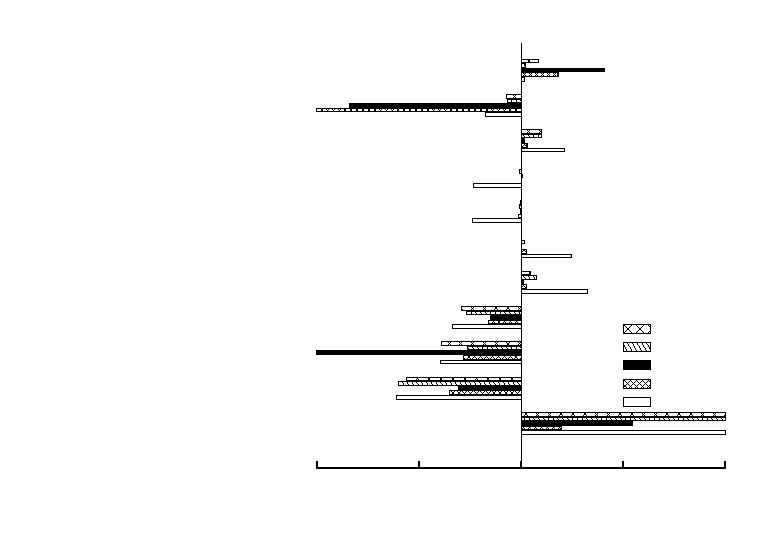
\includegraphics{ch-dynamics/CEMA_80}}%
    \gplfronttext
  \end{picture}%
\endgroup
}
  \normalsize
  \caption{Normalized participation index at $2.4$ and $8.0$ m/s.  Sampled locations are delineated in Fig.~\ref{fig:HRR_V}.}
  \label{fig:CEMA_V}
\end{figure}

At $2.4$ m/s, the dominant reactions along $Z_{\rm st}$ and $Z = 0.2$ iso-contours evolve in similar ways: upstream of the tribrachial structure (point A, B, and D), low temperature chemistry, characterized by reactions involving CH$_3$OCH$_2$O$_2$ radicals, are active.  Due to the high diffusivity of H radical and the elevated pressure, the H radical recombination reaction (H + O$_2$ + M $\Longleftrightarrow$ HO$_2$ + M) are important.  At the most reactive region (point C and E), the hydrogen branching reaction (H + O$_2$ $\Longleftrightarrow$ O + OH) becomes the most important chain branching reaction, indicating the transition to high temperature chemistry.

On the contrary, for the $8.0$ m/s case, while the low temperature chemistry is still active upstream of the multibrachial structure , the dominant chain branching reaction is the hydrogen peroxide branching reaction (H$_2$O$_2$ + M $\Longleftrightarrow$ OH + OH + M).  Moreover, the dominant reactions along $Z_{\rm st}$ and $Z = 0.2$ iso-contours evolve in different ways: along $Z = 0.2$ iso-contour, from point D to E, the hydrogen peroxide branching reaction is always the dominate reaction, indicating the role of low-to-intermediate temperature autoignition chemistry~\cite{westbrook00}.  However, although this is the case at point A on $Z_{\rm st}$ iso-contour, the H radical chain branching reaction becomes dominate at point C, the most reactive zone, indicating that the dominate chemical pathways shift high temperature chemistry.  

\subsection{Stabilization Mechanism} 
The above CEMA results have demonstrated the importance of autoignition chemistry in the multibrachial structure.  However, further analysis is still need to elucidate the role that autoignition chemistry plays in the stabilization mechanism.  As demonstrated previously~\cite{deng15}, the Lagrangian Flamelet Analysis (LFA)~\cite{pitsch98a} utilizes the initial conditions given by the two-dimensional computation to provide the time history of the one-dimensional inhomogeneous autoignition.  As only the diffusion processes parallel to the mixture fraction gradient direction are allowed, the comparison of this one-dimensional flamelet and the two-dimensional computation gives the relative importance of the transport parallel and perpendicular to the mixture fraction gradient, thus the relative importance of inhomogeneous autoignition and premixed flame propagation to the stabilization mechanism.

Specifically, species mass fractions and temperature were sampled ten times of the wall thickness downstream of the inlet to avoid the influence from the recirculation zone as the initial condition for LFA.  The time history of the scalar dissipation rate was sampled along $Z_{\rm st}$ iso-contour from the two-dimensional computation and feed into LFA as well.  Details about the governing equations can be found in Pitsch \emph{et al.}~\cite{pitsch98a} and the previous work~\cite{deng15}.

The Lagrangian time history profiles of the two-dimensional computation and one-dimensional LFA are shown in Fig.~\ref{fig:LFA_V}.  For each inlet velocity case, the temperature profiles are compared along $Z_{\rm st}$, $Z = 0.2$, and $Z = 0.3$.  

For the $2.4$ m/s case, LFA fails to match the two-dimensional computation at all three mixture fractions, indicating that the transport processes perpendicular to the mixture fraction gradient is crucial, which further indicates that flame propagation is the dominant stabilization mechanism.

At $3.2$ m/s, LFA is slightly lagging behind the two-dimensional computation at $Z_{\rm st}$, but correlates well with at $Z = 0.2$ and $Z = 0.3$.  Recalling the heat release profile in Fig.~\ref{fig:HRR_V}, these results indicate that the tetrabrachial structure consists of a tribrachial structure, at which flame propagation is not negligible, and the richer branch that intersects with the tribrachial flame is an autoignition front, whose response is well captured with the one-dimensional inhomogeneous flamelet model.  As a consequence, the stabilization of the $3.2$ m/s is characterized as a mixed mode of inhomogeneous autoignition and premixed flame propagation.

At $8.0$ m/s, LFA agrees well with the two-dimensional computation at all there mixture fractions, indicating that the transport processes perpendicular to the mixture fraction gradient are negligible compared to the parallel direction.  Therefore, the stabilization mechanism is characterized as inhomogeneous autoignition.

\begin{figure}
  \centering
  \scriptsize
  \resizebox{0.8\textwidth}{!}{% GNUPLOT: LaTeX picture with Postscript
\begingroup
  \makeatletter
  \providecommand\color[2][]{%
    \GenericError{(gnuplot) \space\space\space\@spaces}{%
      Package color not loaded in conjunction with
      terminal option `colourtext'%
    }{See the gnuplot documentation for explanation.%
    }{Either use 'blacktext' in gnuplot or load the package
      color.sty in LaTeX.}%
    \renewcommand\color[2][]{}%
  }%
  \providecommand\includegraphics[2][]{%
    \GenericError{(gnuplot) \space\space\space\@spaces}{%
      Package graphicx or graphics not loaded%
    }{See the gnuplot documentation for explanation.%
    }{The gnuplot epslatex terminal needs graphicx.sty or graphics.sty.}%
    \renewcommand\includegraphics[2][]{}%
  }%
  \providecommand\rotatebox[2]{#2}%
  \@ifundefined{ifGPcolor}{%
    \newif\ifGPcolor
    \GPcolortrue
  }{}%
  \@ifundefined{ifGPblacktext}{%
    \newif\ifGPblacktext
    \GPblacktexttrue
  }{}%
  % define a \g@addto@macro without @ in the name:
  \let\gplgaddtomacro\g@addto@macro
  % define empty templates for all commands taking text:
  \gdef\gplbacktext{}%
  \gdef\gplfronttext{}%
  \makeatother
  \ifGPblacktext
    % no textcolor at all
    \def\colorrgb#1{}%
    \def\colorgray#1{}%
  \else
    % gray or color?
    \ifGPcolor
      \def\colorrgb#1{\color[rgb]{#1}}%
      \def\colorgray#1{\color[gray]{#1}}%
      \expandafter\def\csname LTw\endcsname{\color{white}}%
      \expandafter\def\csname LTb\endcsname{\color{black}}%
      \expandafter\def\csname LTa\endcsname{\color{black}}%
      \expandafter\def\csname LT0\endcsname{\color[rgb]{1,0,0}}%
      \expandafter\def\csname LT1\endcsname{\color[rgb]{0,1,0}}%
      \expandafter\def\csname LT2\endcsname{\color[rgb]{0,0,1}}%
      \expandafter\def\csname LT3\endcsname{\color[rgb]{1,0,1}}%
      \expandafter\def\csname LT4\endcsname{\color[rgb]{0,1,1}}%
      \expandafter\def\csname LT5\endcsname{\color[rgb]{1,1,0}}%
      \expandafter\def\csname LT6\endcsname{\color[rgb]{0,0,0}}%
      \expandafter\def\csname LT7\endcsname{\color[rgb]{1,0.3,0}}%
      \expandafter\def\csname LT8\endcsname{\color[rgb]{0.5,0.5,0.5}}%
    \else
      % gray
      \def\colorrgb#1{\color{black}}%
      \def\colorgray#1{\color[gray]{#1}}%
      \expandafter\def\csname LTw\endcsname{\color{white}}%
      \expandafter\def\csname LTb\endcsname{\color{black}}%
      \expandafter\def\csname LTa\endcsname{\color{black}}%
      \expandafter\def\csname LT0\endcsname{\color{black}}%
      \expandafter\def\csname LT1\endcsname{\color{black}}%
      \expandafter\def\csname LT2\endcsname{\color{black}}%
      \expandafter\def\csname LT3\endcsname{\color{black}}%
      \expandafter\def\csname LT4\endcsname{\color{black}}%
      \expandafter\def\csname LT5\endcsname{\color{black}}%
      \expandafter\def\csname LT6\endcsname{\color{black}}%
      \expandafter\def\csname LT7\endcsname{\color{black}}%
      \expandafter\def\csname LT8\endcsname{\color{black}}%
    \fi
  \fi
  \setlength{\unitlength}{0.0500bp}%
  \begin{picture}(8640.00,6048.00)%
    \gplgaddtomacro\gplbacktext{%
      \csname LTb\endcsname%
      \put(6694,4756){\makebox(0,0)[r]{\strut{} 800}}%
      \put(6694,4961){\makebox(0,0)[r]{\strut{} 1200}}%
      \put(6694,5167){\makebox(0,0)[r]{\strut{} 1600}}%
      \put(6694,5372){\makebox(0,0)[r]{\strut{} 2000}}%
      \put(6694,5578){\makebox(0,0)[r]{\strut{} 2400}}%
      \put(6694,5783){\makebox(0,0)[r]{\strut{} 2800}}%
      \put(6826,4536){\makebox(0,0){\strut{} 0}}%
      \put(7137,4536){\makebox(0,0){\strut{} 0.5}}%
      \put(7448,4536){\makebox(0,0){\strut{} 1}}%
      \put(7759,4536){\makebox(0,0){\strut{} 1.5}}%
      \put(8070,4536){\makebox(0,0){\strut{} 2}}%
      \put(5792,5269){\rotatebox{-270}{\makebox(0,0){\strut{}\vspace{-36pt}$T$ [K]}}}%
      \put(7448,4206){\makebox(0,0){\strut{}\vspace{12pt}Time [ms]}}%
      \put(1987,6047){\makebox(0,0)[l]{\strut{}$2.4$ m/s}}%
      \put(4579,6047){\makebox(0,0)[l]{\strut{}$3.2$ m/s}}%
      \put(7170,6047){\makebox(0,0)[l]{\strut{}$8.0$ m/s}}%
      \put(-172,1633){\makebox(0,0)[l]{\strut{}$Z = 0.3$}}%
      \put(-172,3447){\makebox(0,0)[l]{\strut{}$Z = 0.2$}}%
      \put(-172,5261){\makebox(0,0)[l]{\strut{}$Z = Z_{\rm st}$}}%
    }%
    \gplgaddtomacro\gplfronttext{%
    }%
    \gplgaddtomacro\gplbacktext{%
      \csname LTb\endcsname%
      \put(6694,2941){\makebox(0,0)[r]{\strut{} 600}}%
      \put(6694,3147){\makebox(0,0)[r]{\strut{} 1000}}%
      \put(6694,3352){\makebox(0,0)[r]{\strut{} 1400}}%
      \put(6694,3558){\makebox(0,0)[r]{\strut{} 1800}}%
      \put(6694,3763){\makebox(0,0)[r]{\strut{} 2200}}%
      \put(6694,3969){\makebox(0,0)[r]{\strut{} 2600}}%
      \put(6826,2721){\makebox(0,0){\strut{} 0}}%
      \put(7137,2721){\makebox(0,0){\strut{} 0.5}}%
      \put(7448,2721){\makebox(0,0){\strut{} 1}}%
      \put(7759,2721){\makebox(0,0){\strut{} 1.5}}%
      \put(8070,2721){\makebox(0,0){\strut{} 2}}%
      \put(5792,3455){\rotatebox{-270}{\makebox(0,0){\strut{}\vspace{-36pt}$T$ [K]}}}%
      \put(7448,2391){\makebox(0,0){\strut{}\vspace{12pt}Time [ms]}}%
    }%
    \gplgaddtomacro\gplfronttext{%
    }%
    \gplgaddtomacro\gplbacktext{%
      \csname LTb\endcsname%
      \put(6694,1187){\makebox(0,0)[r]{\strut{} 400}}%
      \put(6694,1393){\makebox(0,0)[r]{\strut{} 800}}%
      \put(6694,1598){\makebox(0,0)[r]{\strut{} 1200}}%
      \put(6694,1804){\makebox(0,0)[r]{\strut{} 1600}}%
      \put(6694,2009){\makebox(0,0)[r]{\strut{} 2000}}%
      \put(6694,2215){\makebox(0,0)[r]{\strut{} 2400}}%
      \put(6826,967){\makebox(0,0){\strut{} 0}}%
      \put(7137,967){\makebox(0,0){\strut{} 0.5}}%
      \put(7448,967){\makebox(0,0){\strut{} 1}}%
      \put(7759,967){\makebox(0,0){\strut{} 1.5}}%
      \put(8070,967){\makebox(0,0){\strut{} 2}}%
      \put(5792,1701){\rotatebox{-270}{\makebox(0,0){\strut{}\vspace{-36pt}$T$ [K]}}}%
      \put(7448,637){\makebox(0,0){\strut{}\vspace{12pt}Time [ms]}}%
    }%
    \gplgaddtomacro\gplfronttext{%
    }%
    \gplgaddtomacro\gplbacktext{%
      \csname LTb\endcsname%
      \put(4102,4756){\makebox(0,0)[r]{\strut{} 800}}%
      \put(4102,4961){\makebox(0,0)[r]{\strut{} 1200}}%
      \put(4102,5167){\makebox(0,0)[r]{\strut{} 1600}}%
      \put(4102,5372){\makebox(0,0)[r]{\strut{} 2000}}%
      \put(4102,5578){\makebox(0,0)[r]{\strut{} 2400}}%
      \put(4102,5783){\makebox(0,0)[r]{\strut{} 2800}}%
      \put(4234,4536){\makebox(0,0){\strut{} 0}}%
      \put(4545,4536){\makebox(0,0){\strut{} 0.3}}%
      \put(4856,4536){\makebox(0,0){\strut{} 0.6}}%
      \put(5167,4536){\makebox(0,0){\strut{} 0.9}}%
      \put(5478,4536){\makebox(0,0){\strut{} 1.2}}%
      \put(3200,5269){\rotatebox{-270}{\makebox(0,0){\strut{}\vspace{-36pt}$T$ [K]}}}%
      \put(4856,4206){\makebox(0,0){\strut{}\vspace{12pt}Time [ms]}}%
    }%
    \gplgaddtomacro\gplfronttext{%
    }%
    \gplgaddtomacro\gplbacktext{%
      \csname LTb\endcsname%
      \put(4102,2941){\makebox(0,0)[r]{\strut{} 600}}%
      \put(4102,3147){\makebox(0,0)[r]{\strut{} 1000}}%
      \put(4102,3352){\makebox(0,0)[r]{\strut{} 1400}}%
      \put(4102,3558){\makebox(0,0)[r]{\strut{} 1800}}%
      \put(4102,3763){\makebox(0,0)[r]{\strut{} 2200}}%
      \put(4102,3969){\makebox(0,0)[r]{\strut{} 2600}}%
      \put(4234,2721){\makebox(0,0){\strut{} 0}}%
      \put(4545,2721){\makebox(0,0){\strut{} 0.3}}%
      \put(4856,2721){\makebox(0,0){\strut{} 0.6}}%
      \put(5167,2721){\makebox(0,0){\strut{} 0.9}}%
      \put(5478,2721){\makebox(0,0){\strut{} 1.2}}%
      \put(3200,3455){\rotatebox{-270}{\makebox(0,0){\strut{}\vspace{-36pt}$T$ [K]}}}%
      \put(4856,2391){\makebox(0,0){\strut{}\vspace{12pt}Time [ms]}}%
    }%
    \gplgaddtomacro\gplfronttext{%
    }%
    \gplgaddtomacro\gplbacktext{%
      \csname LTb\endcsname%
      \put(4102,1187){\makebox(0,0)[r]{\strut{} 400}}%
      \put(4102,1393){\makebox(0,0)[r]{\strut{} 800}}%
      \put(4102,1598){\makebox(0,0)[r]{\strut{} 1200}}%
      \put(4102,1804){\makebox(0,0)[r]{\strut{} 1600}}%
      \put(4102,2009){\makebox(0,0)[r]{\strut{} 2000}}%
      \put(4102,2215){\makebox(0,0)[r]{\strut{} 2400}}%
      \put(4234,967){\makebox(0,0){\strut{} 0}}%
      \put(4545,967){\makebox(0,0){\strut{} 0.3}}%
      \put(4856,967){\makebox(0,0){\strut{} 0.6}}%
      \put(5167,967){\makebox(0,0){\strut{} 0.9}}%
      \put(5478,967){\makebox(0,0){\strut{} 1.2}}%
      \put(3200,1701){\rotatebox{-270}{\makebox(0,0){\strut{}\vspace{-36pt}$T$ [K]}}}%
      \put(4856,637){\makebox(0,0){\strut{}\vspace{12pt}Time [ms]}}%
    }%
    \gplgaddtomacro\gplfronttext{%
    }%
    \gplgaddtomacro\gplbacktext{%
      \csname LTb\endcsname%
      \put(1510,4756){\makebox(0,0)[r]{\strut{} 800}}%
      \put(1510,4961){\makebox(0,0)[r]{\strut{} 1200}}%
      \put(1510,5167){\makebox(0,0)[r]{\strut{} 1600}}%
      \put(1510,5372){\makebox(0,0)[r]{\strut{} 2000}}%
      \put(1510,5578){\makebox(0,0)[r]{\strut{} 2400}}%
      \put(1510,5783){\makebox(0,0)[r]{\strut{} 2800}}%
      \put(1642,4536){\makebox(0,0){\strut{} 0}}%
      \put(1953,4536){\makebox(0,0){\strut{} 0.3}}%
      \put(2264,4536){\makebox(0,0){\strut{} 0.6}}%
      \put(2575,4536){\makebox(0,0){\strut{} 0.9}}%
      \put(2886,4536){\makebox(0,0){\strut{} 1.2}}%
      \put(608,5269){\rotatebox{-270}{\makebox(0,0){\strut{}\vspace{-36pt}$T$ [K]}}}%
      \put(2264,4206){\makebox(0,0){\strut{}\vspace{12pt}Time [ms]}}%
    }%
    \gplgaddtomacro\gplfronttext{%
    }%
    \gplgaddtomacro\gplbacktext{%
      \csname LTb\endcsname%
      \put(1510,2941){\makebox(0,0)[r]{\strut{} 600}}%
      \put(1510,3147){\makebox(0,0)[r]{\strut{} 1000}}%
      \put(1510,3352){\makebox(0,0)[r]{\strut{} 1400}}%
      \put(1510,3558){\makebox(0,0)[r]{\strut{} 1800}}%
      \put(1510,3763){\makebox(0,0)[r]{\strut{} 2200}}%
      \put(1510,3969){\makebox(0,0)[r]{\strut{} 2600}}%
      \put(1642,2721){\makebox(0,0){\strut{} 0}}%
      \put(1953,2721){\makebox(0,0){\strut{} 0.3}}%
      \put(2264,2721){\makebox(0,0){\strut{} 0.6}}%
      \put(2575,2721){\makebox(0,0){\strut{} 0.9}}%
      \put(2886,2721){\makebox(0,0){\strut{} 1.2}}%
      \put(608,3455){\rotatebox{-270}{\makebox(0,0){\strut{}\vspace{-36pt}$T$ [K]}}}%
      \put(2264,2391){\makebox(0,0){\strut{}\vspace{12pt}Time [ms]}}%
    }%
    \gplgaddtomacro\gplfronttext{%
    }%
    \gplgaddtomacro\gplbacktext{%
      \csname LTb\endcsname%
      \put(1510,1187){\makebox(0,0)[r]{\strut{} 400}}%
      \put(1510,1393){\makebox(0,0)[r]{\strut{} 800}}%
      \put(1510,1598){\makebox(0,0)[r]{\strut{} 1200}}%
      \put(1510,1804){\makebox(0,0)[r]{\strut{} 1600}}%
      \put(1510,2009){\makebox(0,0)[r]{\strut{} 2000}}%
      \put(1510,2215){\makebox(0,0)[r]{\strut{} 2400}}%
      \put(1642,967){\makebox(0,0){\strut{} 0}}%
      \put(1953,967){\makebox(0,0){\strut{} 0.3}}%
      \put(2264,967){\makebox(0,0){\strut{} 0.6}}%
      \put(2575,967){\makebox(0,0){\strut{} 0.9}}%
      \put(2886,967){\makebox(0,0){\strut{} 1.2}}%
      \put(608,1701){\rotatebox{-270}{\makebox(0,0){\strut{}\vspace{-36pt}$T$ [K]}}}%
      \put(2264,637){\makebox(0,0){\strut{}\vspace{12pt}Time [ms]}}%
      \put(4147,242){\makebox(0,0)[l]{\strut{}2D-CFD}}%
      \put(5270,242){\makebox(0,0)[l]{\strut{}1D-LFA}}%
    }%
    \gplgaddtomacro\gplfronttext{%
      \csname LTb\endcsname%
      \put(3646,253){\makebox(0,0)[r]{\strut{} }}%
      \csname LTb\endcsname%
      \put(4765,253){\makebox(0,0)[r]{\strut{}    }}%
    }%
    \gplbacktext
    \put(0,0){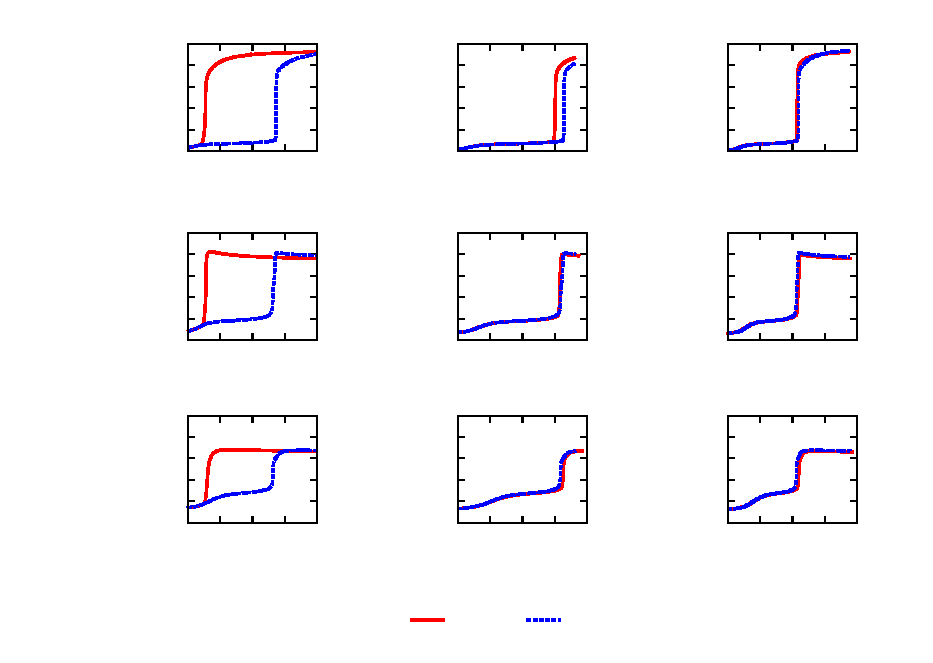
\includegraphics{ch-dynamics/LFA_V}}%
    \gplfronttext
  \end{picture}%
\endgroup
}
  \normalsize
  \vspace{-0.2in}
  \caption{Comparison between NGA and LFA results.}
  \label{fig:LFA_V}
\end{figure}

\subsection{Autoignition Flame Interaction}

As shown by LFA, under some conditions, inhomogeneous autoignition and premixed flame propagation both contribute to the stabilization, resulting in the multimode stabilized regime.  The interaction between autoignition and flame propagation is complex: if the thermal structure is mainly \emph{kinetically} stabilized, heat and radicals generated by autoignition can modify downstream thermal and chemical environment, thus local flame speeds.  On the contrary, if mainly \emph{kinematically} stabilized, heat and radicals generated by flame can back diffuse upstream, modifying the reactivity upstream.  

To demonstrate these complex interactions and understand the transition between \emph{kinetic} to \emph{kinematic} stabilization, the LFA results for the $2.4$ m/s case were further analyzed.  As shown in Fig.~\ref{fig:LFA_V}, if there was a \emph{kinetically} stabilized inhomogeneous autoignition front, this front would stabilize further downstream than the \emph{kinematically} stabilized flame front.  Although not shown, the CEMA samplings of these LFA solutions show the same evolution of the controlling chemistry as the $8.0$ m/s case.  Especially, the low-to-intermediate temperature hydrogen peroxide chain branching reaction is the dominant reaction that leads to the autoignition.  Therefore, the nature and the qualitative structures of the inhomogeneous autoignition fronts ,predicted by LFA in Fig.~\ref{LFA_V} for the two lower inlet velocity cases, are essentially the same as the $8.0$ m/s case.  A general description of the initiation of these multibrachial inhomogeneous autoignition front is that, due to radical accumulation and heat release, the controlling chemistry shifts from low temperature chemistry to intermediate temperature chemistry.  At $Z_{\rm st}$, higher temperature and more oxidizer supply enables the dominant chemistry further transits to high temperature chemistry.   

However, after the initiation of this inhomogeneous autoignition front, the stabilization of the final structure depends on the residence time, which is determined by the inlet velocity of the current study.  At $8.0$ m/s, the flow residence time is very short, such that heat and radical back diffusion processes from the autoignition front to upstream are not able to keep up with the convection; therefore, the reacting front is \emph{kinetically} stabilized.  At $3.2$ m/s, the flow residence time is longer, allowing for back diffusion to some extent, such that the reacting front can propagate upstream.  However, the propagation speed of the reacting front is different as the composition and temperature varies.  As a consequence, around $Z_{\rm st}$, where higher temperature and nearly stoichiometry enables higher flame speed, the propagation of the reacting front balances the incoming flow velocity, while such balance fails at richer mixture fractions and \emph{kinetic} stabilization is dominant.  At $2.4$ m/s, back diffusion is important to all mixture fractions, such that the reacting front propagates upstream at the local flame speed, determined by the local composition and temperature.  Due to increased temperature and species stratification and less accumulation from autoignition, the propagation speed of this reacting front slows down as it moves upstream and eventually balances the local flow velocity.  The structure of this \emph{kinematically} stabilized reacting front, which is generally tribrachial, is therefore determined by the variation of the local flame speed, rather than the inhomogeneous autoignition.      

% for the journal paper: add Zeldovich propagation and show the flame supported autoignition (HRR) and 1D sampling from the 2D stats to show that the autoignition front is not part of the flame.   

        
%====================================================================
\section{Stabilization Regime Diagram}

The above sections have demonstrated the residence time effects on the thermal and chemical structure of the lifted coflow flames and the stabilization mechanisms.  Combining with the chemical time effects demonstrated by changing the coflow boundary temperature in previous study~\cite{deng15}, a two-dimensional stabilization regime diagram is proposed, as shown in Fig.~\ref{fig:2D-regime}.  

\begin{figure}
  \centering
  \scriptsize
  \vspace{-0.1in}
  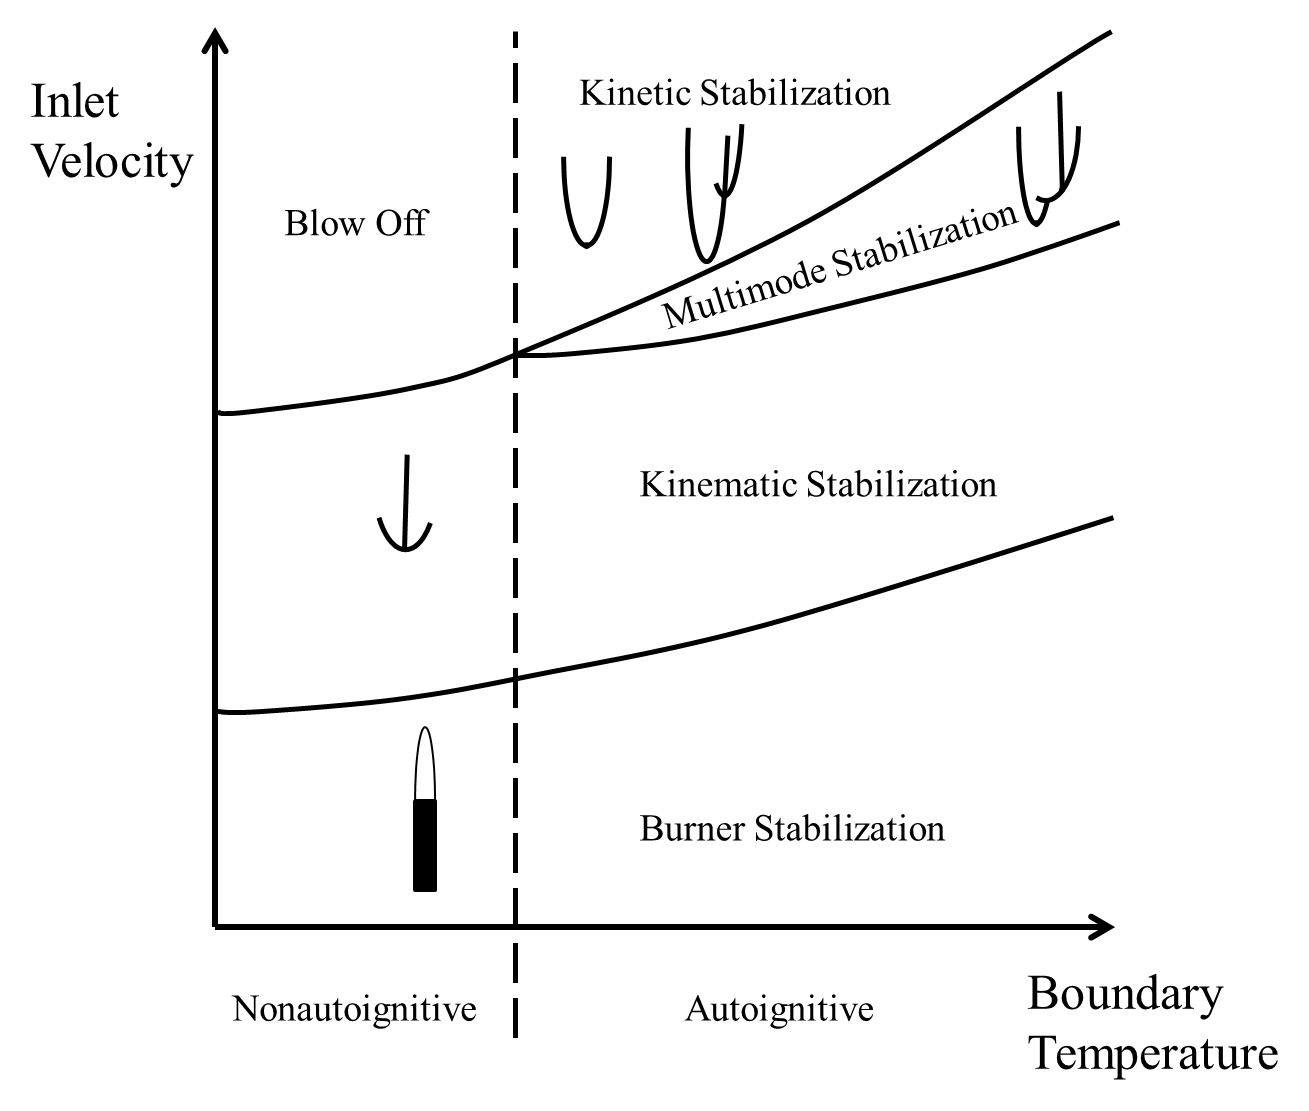
\includegraphics[width=0.6\textwidth]{2D-regime.png}
  \normalsize
  \vspace{-0.1in}
  \caption{A qualitative regime diagram for the stabilization mechanisms as the boundary temperature and inlet velocity vary. }
  \label{fig:2D-regime}
\end{figure}

Qualitatively, when the boundary temperature is not high enough to activate autoignition, the lifted flame appears as the classical triple flame and is \emph{kinematic} stabilized.  When the inlet velocity is below or above certain threshold values, the triple flame becomes attached to the burner or is blown off, respectively.  

As the boundary temperature is elevated to activate autoignition, the transition of the stabilization mechanism for increasing inlet velocity follows the observation made in the current study: from burner stabilization to \emph{kinematic} balance between flame speed and incoming flow velocity, to multimode stabilization influenced by both flame propagation and inhomogeneous autoignition, and finally to \emph {kinetic} stabilization governed by inhomogeneous autoignition.  It is expected that the crossover velocities between regimes increase with increasing boundary temperature, for flame speed generally increases at higher temperature.  However, it is difficult to quantify these boundaries, as local composition and temperature vary streamwise, and therefore, the reference flame speed cannot be calculated based on the upstream boundary conditions.  Furthermore, local flame front curvature, cross-stream species stratification, and flow divergence approaching the flame front also modifies the flame speed.  As a consequence, only a qualitative trend is demonstrated in Fig.~\ref{fig:2D-regime}.  

Similarly, if the boundary temperature increases at fixed inlet velocity, a transition from blow off to burner stabilized regimes is achieved moving horizontally across the regime diagram, which was discussed in the previous work~\cite{deng15}.     

%====================================================================

\section{Conclusions}

In the present work, axisymmetric two-dimensional laminar nonpremixed DME lifted coflow flames at elevated temperature and pressure were computed.  The residence time effects on the structure and stabilization mechanism were demonstrated by changing the inlet velocities, while keeping the coflow boundary temperature constant.

The heat release rate profiles were examined to describe the thermal structure.  Computational Explosive Mode Analysis (CEMA) was adopted to demonstrate the evolution of the controlling chemistry.  Moreover, the one-dimensional Lagrangian Flamelet Analysis that captures the inhomogeneous autoignition was adopted to demonstrate the dominant transport directions, and therefore determine the dominant combustion mode and stabilization mechanism.

At $2.4$ m/s, the lifted flame appears to be the classical triple flame, stabilized by the balance between the local flame speed and incoming flow velocity, and therefore is characterized as \emph {kinematically} stabilized.  As inlet velocity increase, such balance cannot be achieved at certain mixture fractions, instead, inhomogeneous autoignition is the dominant combustion mode.  As a consequence, the multibrachial structure is stabilized by both premixed flame propagation and inhomogeneous autoignition and is characterized as multimode stabilized.  At $8.0$ m/s, the \emph{kinematic} balance cannot be achieved anywhere in the flow field, due to reduced residence time.  A \emph {kinetically} stabilized inhomogeneous autoignition front is formed, where diffusion processes along mixture fraction iso-contours are negligible compared to the gradient direction.

Combined with the extended stabilization regimes demonstrated in the previous study~\cite{deng15}, an extended two-dimensional stabilization regime diagram was obtained in the present work, considering both residence time (inlet velocity) and chemical time (coflow boundary temperature) effects.  

%====================================================================

\section{Acknowledgements}

\textcolor{red}{TBD}

%====================================================================
\bibliographystyle{wssci}
\bibliography{NCM_Jet} 

\end{document}
